\chapter{Lezione 19}
\label{chap:lezione_19}

\begin{flushright}
\textit{Data: 26/11/2025}
\end{flushright}


\noindent Continuiamo la nostra analisi della teoria di campo scalare con interazione quartica ~$\varphi^4$.
L'obiettivo è calcolare le funzioni di correlazione in modo perturbativo rispetto alla costante di accoppiamento $g$.

\subsubsection{Recap del Primo Ordine}
Al primo ordine (ordine $g$), abbiamo incontrato il diagramma "Tadpole".
L'espansione coinvolge il calcolo del valore di aspettazione Gaussiano dei campi.
Per la funzione di correlazione a due punti $\langle \varphi(x) \varphi(0) \rangle$, questo ordine coinvolge un singolo vertice interno di interazione.

Ora ci muoviamo verso l'espansione al \textbf{secondo ordine} (ordine $g^2$).
Calcoleremo il numeratore dell'espansione perturbativa, limitandoci ai \textbf{diagrammi connessi}, poiché i diagrammi disconnessi si cancellano con il denominatore (la funzione di partizione $\mathcal{Z}$), come visto nel Teorema dei Cluster Connessi.

\section{Il Contributo al Secondo Ordine}

Al secondo ordine, abbiamo due vertici di interazione.
Denotiamo i punti esterni come $x$ e $0$, e le variabili di integrazione interne (i vertici) come $y_1$ e $y_2$.
Il termine che dobbiamo valutare è proporzionale a:

\begin{equation}
    \frac{1}{2!} (-g)^2 \int dy_1 dy_2 \langle \varphi(x) \varphi(0) \varphi^4(y_1) \varphi^4(y_2) \rangle_0
\end{equation}

dove $\langle \dots \rangle_0$ denota il valore di aspettazione Gaussiano (nella teoria libera).


\noindent Abbiamo un totale di 10 campi da contrarre:
\begin{itemize}
    \item 2 campi esterni: $\varphi(x), \varphi(0)$;
    \item 8 campi interni: 4 al vertice $y_1$ e 4 al vertice $y_2$.
\end{itemize}

\noindent Il numero totale di modi per contrarre questi campi in coppie è dato dal Teorema di Wick come il doppio fattoriale $(10-1)!! = 945$.
Tuttavia, siamo interessati solo alle topologie distinte \textbf{connesse}.

\subsubsection{ Fattore di Simmetria:}
Consideriamo la contrazione del campo esterno $\varphi(x)$ con un campo interno. Possiamo connettere $\varphi(x)$ a un campo nel vertice $y_1$ (4 modi) oppure a un campo nel vertice $y_2$ (4 modi). A causa della simmetria tra le variabili di integrazione $y_1$ e $y_2$, queste due scelte sono equivalenti.
Fissando la connessione a $y_1$, moltiplichiamo per un fattore 2, il quale cancella esattamente il fattore $1/2!$ proveniente dall'espansione di Taylor.

Pertanto, assumiamo che $x$ si connetta a $y_1$ e non dividiamo più per $2!$.

\hfill

\noindent Esistono due topologie connesse distinte per la funzione a due punti all'ordine $g^2$: il diagramma "Cactus" e il diagramma "Hamburger".

\subsubsection{Il Diagramma Cactus (Double Tadpole)}


Questo diagramma è "riducibile a una particella" (one-particle reducible), ovvero può essere separato in due parti disconnesse tagliando una singola linea interna.

\begin{itemize}
    \item \textbf{Struttura:}
       \begin{center}
    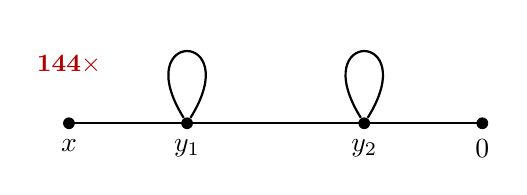
\begin{tikzpicture}[scale=1.5, 
        vertex/.style={circle, fill=black, inner sep=1.5pt},
        label_node/.style={font=\small},
        multiplicity/.style={font=\small\bfseries, color=red!70!black}
    ]
    \begin{scope}[shift={(0,0)}]
        
        
        % Linea di base
        \draw[thick] (0,0) -- (3.5,0);
        
        % Vertici
        \node[vertex, label=below:$x$] (x) at (0,0) {};
        \node[vertex, label=below:$y_1$] (y1) at (1,0) {};
        \node[vertex, label=below:$y_2$] (y2) at (2.5,0) {};
        \node[vertex, label=below:$0$] (z) at (3.5,0) {};
        
        % Loops (Bools)
        \draw[thick] (y1) .. controls (0.5, 0.8) and (1.5, 0.8) .. (y1);
        \draw[thick] (y2) .. controls (2.0, 0.8) and (3.0, 0.8) .. (y2);
        
        % Molteplicità
        \node[multiplicity] at (0, 0.5) {$\mathbf{144 \times}$};
        
     
    \end{scope}
    \end{tikzpicture}
    \end{center}
    
    \item \textbf{Calcolo della Molteplicità:}
    \begin{enumerate}
        \item Connettere $\varphi(x)$ a $y_1$: \textbf{4} modi.
        \item Connettere $\varphi(0)$ a $y_2$: \textbf{4} modi.
        \item Formare un loop su $y_1$ (contrarre 2 dei restanti 3 campi): \textbf{3} modi.
        \item Formare un loop su $y_2$ (contrarre 2 dei restanti 3 campi): \textbf{3} modi.
        \item Connettere il campo rimanente in $y_1$ al campo rimanente in $y_2$: \textbf{1} modo.
    \end{enumerate}
    
    \item \textbf{Molteplicità Totale:} $4 \times 4 \times 3 \times 3 \times 1 = \mathbf{144}$.
\end{itemize}

\subsubsection{Il Diagramma Hamburger (Setting Sun)}


Questo diagramma connette $y_1$ e $y_2$ tramite tre linee interne. Non può essere separato tagliando una singola linea (è irriducibile).

\begin{itemize}
    \item \textbf{Struttura:} 
      \begin{center}
    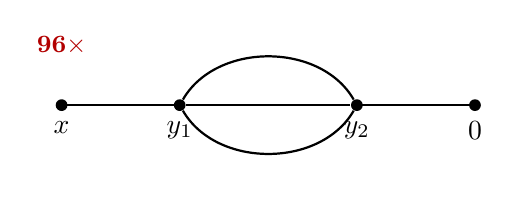
\begin{tikzpicture}[scale=1.5, 
        vertex/.style={circle, fill=black, inner sep=1.5pt},
        label_node/.style={font=\small},
        multiplicity/.style={font=\small\bfseries, color=red!70!black}
    ]
    \begin{scope}[shift={(0,0)}]
      
        % Gambe esterne
        \draw[thick] (0,0) -- (1,0); 
        \draw[thick] (2.5,0) -- (3.5,0); 
        
        % Vertici
        \node[vertex, label=below:$x$] (x) at (0,0) {};
        \node[vertex, label=below:$y_1$] (y1) at (1,0) {};
        \node[vertex, label=below:$y_2$] (y2) at (2.5,0) {};
        \node[vertex, label=below:$0$] (z) at (3.5,0) {};
        
        % 3 Linee interne (Tramonto)
        \draw[thick] (y1) -- (y2);                 % linea centrale
        \draw[thick] (y1) to[bend left=60] (y2);   % arco sopra
        \draw[thick] (y1) to[bend right=60] (y2);  % arco sotto
        
        % Molteplicità
        \node[multiplicity] at (0, 0.5) {$\mathbf{96 \times}$};
        
        
        
    \end{scope}
    \end{tikzpicture}
    \end{center}
    
    \item \textbf{Calcolo della Molteplicità:}
    \begin{enumerate}
        \item Connettere $\varphi(x)$ a $y_1$: \textbf{4} modi.
        \item Connettere $\varphi(0)$ a $y_2$: \textbf{4} modi.
        \item Connettere i restanti 3 campi in $y_1$ ai 3 campi in $y_2$: ci sono $3! = \mathbf{6}$ modi.
    \end{enumerate}
    
    \item \textbf{Molteplicità Totale:} $4 \times 4 \times 6 = \mathbf{96}$.
\end{itemize}

\section{Regole di Feynman Generali per la Molteplicità}

Invece di contare le contrazioni manualmente caso per caso, possiamo utilizzare i fattori di simmetria.

\begin{tcolorbox}[colback=yellow!25, colframe=yellow!75!orange, coltitle=black, title=\textbf{Regola della Molteplicità}]

Per un diagramma con $N$ vertici nella teoria $\varphi^4$:
\begin{equation}
    \text{Molteplicità} = \frac{(24)^N}{S}
\end{equation}
Dove:
\begin{itemize}
    \item $24 = 4!$ deriva dalla costante di accoppiamento del vertice $\frac{g}{4!}$.
    \item $S$ è il \textbf{Fattore di Simmetria} del diagramma (il numero di permutazioni delle linee interne o dei vertici che lasciano il diagramma invariato).
\end{itemize}
\end{tcolorbox}

\subsection*{Applicazione della Regola}
\begin{itemize}
    \item \textbf{Diagramma Cactus:}
    \begin{itemize}
        \item Fattore base: $24^2$ (due vertici).
        \item Fattore di simmetria $S$: Ogni loop tadpole ha una simmetria di 2 (possiamo scambiare i due estremi della linea che forma il loop). Avendo due tadpole, $S = 2 \times 2 = 4$.
        \item Risultato: $\frac{24 \times 24}{4} = 144$. Coincide con il conteggio delle contrazioni.
    \end{itemize}
    
    \item \textbf{Diagramma Hamburger:}
    \begin{itemize}
        \item Fattore base: $24^2$.
        \item Fattore di simmetria $S$: Ci sono 3 linee parallele tra $y_1$ e $y_2$. Possiamo permutare queste linee in $3! = 6$ modi senza cambiare la topologia.
        \item Risultato: $\frac{24 \times 24}{6} = 96$. Coincide con il conteggio delle contrazioni.
    \end{itemize}
\end{itemize}

\section{Il Controllo Zero-Dimensionale}

Un metodo potente per verificare se abbiamo individuato tutti i diagrammi e se le molteplicità sono corrette è utilizzare la \textbf{Teoria di Campo Zero-Dimensionale}.
In 0-D, l'integrale funzionale si riduce a un integrale standard su una variabile $z$:

\begin{equation}
    \mathcal{Z} = \int dz \, e^{-S(z)}, \quad S(z) = \frac{z^2}{2} + \frac{g}{4!} z^4
\end{equation}

\noindent La somma di tutte le molteplicità a un dato ordine $k$ deve eguagliare il coefficiente di $g^k$ nell'espansione perturbativa del valore di aspettazione $\langle z^2 \rangle$.

\begin{equation}
    \langle z^2 \rangle = \frac{\int dz \, z^2 \, e^{-\frac{z^2}{2} - \frac{g}{24}z^4}}{\int dz \, e^{-\frac{z^2}{2} - \frac{g}{24}z^4}}
\end{equation}

\noindent Espandendo l'esponenziale e calcolando i momenti usando l'integrazione Gaussiana ($\langle z^{2n} \rangle_0 = (2n-1)!!$), possiamo verificare che la somma dei pesi dei diagrammi ($144 + 96 + \dots$) corrisponda esattamente ai coefficienti dell'espansione esatta.